\section{Introduction}
In this assignment, we will firstly carry out a regression task using the \textit{Glass Identification} dataset. Subsequently, we will proceed with a classification task using the same dataset. Both of these tasks will be statistically evaluated using relevant measures and methods. In the end, the results of said tasks will be discussed and compared with the results of another paper on the same dataset. 

\section{Regression (part a)}
% Before doing any actual work on our dataset we start of by partitioning off $\approx 5\%$ of the full dataset as to have a validation set that hasnt been seen by any of the models during training, neither as a target or input. This is done to ensure proper validation. \color[red]{den her ide er scrapped for nu}

In the first part of this assignment, we will use regression to predict the value of the \textit{refractive index} (\texttt{RI}) of the glass where the remaining attributes detailing the chemical composition of the glass will be used as input. \\ 

We will lead off by doing forward feature selection using k-fold cross-validation, in an attempt to get the best variables for our linear regression and simultaneously reduce the chance of the model overfitting.\\
\begin{figure}[H]
    \centering
    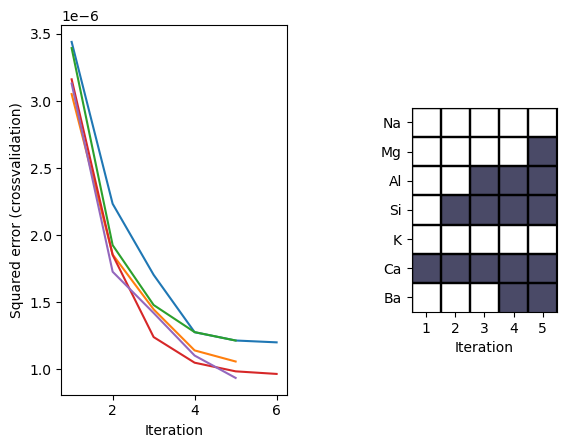
\includegraphics[width=12cm]{images/featureselection.png}
    \caption{Feature selection}
    \label{fig:fig_select}
\end{figure}
As can be seen, we are left with two less variables and we can therefore reduce the dimensionality of our dataset from the get-go. Over several iterations of the feature selections we saw different combinations of features, but this combination was the most prevalent, and we will save this later to evaluate against other models. This also means that we do not utilize the feature selection when going into the regularization \\ \color[red]{Er meget usikker på det her, men giver fucking 0 mening at bruge feature selectionen ind i regularization og har kun gjort det fordi rapporten ligger op til det}

We now want to accommodate for overfitting using regularization. As such we start off by standardizing the full data-set such that the mean of all the variable is 0 and the standard deviation is 1. \color[red]{It is worth noting that the helper function "rlr_validate" also standardizes its internal data partitions as a part of kfold cross-validation when it selects values of $\lambda$} \\
To the further prevent over-fitting we introduce a regularization parameter $\lambda$, which we determine by testing different values and evaluate using the generalization error.
\begin{figure}[H]
    \centering
    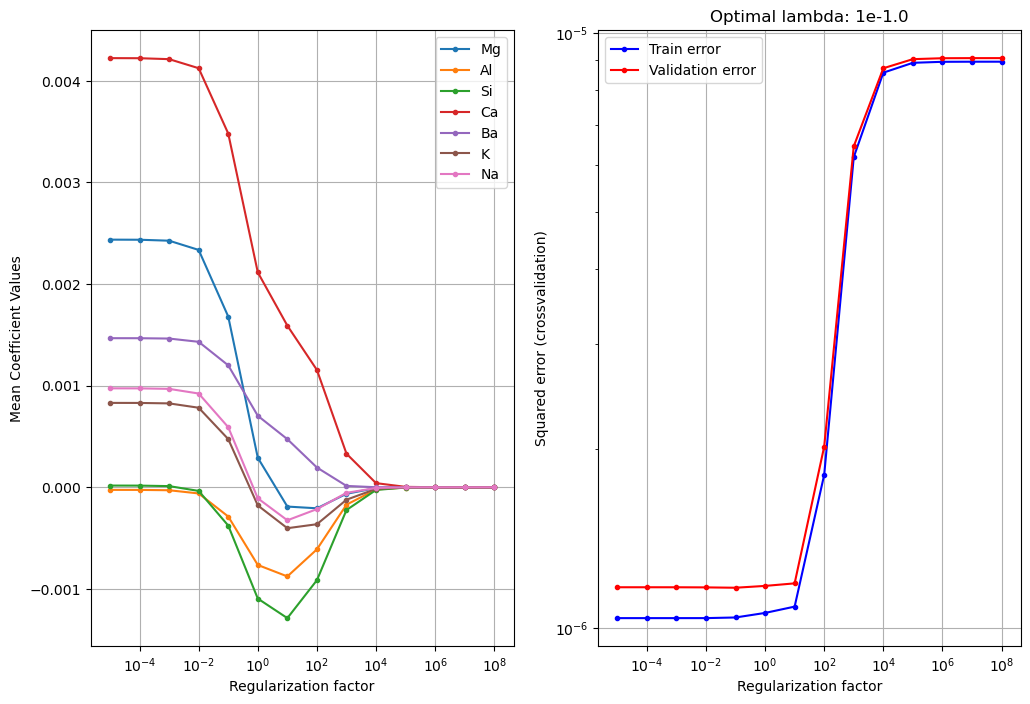
\includegraphics[width=15cm]{images/regularization.png}
    \caption{Plot of the Mean Coefficient Values and Squared error as a function of the regularization factor}
    \label{fig:regu_plot}
\end{figure}
While it doesn't seem that a regularization factor ends up impacting the regression itself, its worth noting how the offset of namely Al and Si gives their coefficient a weight different than 0 and thus we will go with the found optimal regularization factor of $\lambda = 1\cdot 10^{-1} = 0.1$. \\
Again its worth noting that for every K-fold run we test, we tend to get different optimal values of $\lambda$, but the chosen one, was the most occuring one. This might be due to both our dataset being on the smaller side, or that our dataset simply is meant for regression.\\

To understand how the model now do the regression we can simply look at the corresponding weights of the optimal $\lambda$.(We have chosen not to include that weights themselves as they change too much over each run).\\We these values we simply linearly apply them to an new data observation as a matter of matrix multiplication and as such calculate the regression target "RI" using these.\\
\\
\\


\section{Regression (part b)}
